\documentclass{tufte-handout}

\title{Introductory Python: List Comprehensions }

\author[Schultz]{NYC Data Science Academy\\Dr. Anthony Schultz}

\date{January 10, 2017} % without \date command, current date is supplied

%\geometry{showframe} % display margins for debugging page layout

\usepackage{graphicx} % allow embedded images
  \setkeys{Gin}{width=\linewidth,totalheight=\textheight,keepaspectratio}
  \graphicspath{{graphics/}} % set of paths to search for images
\usepackage{amsmath}  % extended mathematics
\usepackage{booktabs} % book-quality tables
\usepackage{units}    % non-stacked fractions and better unit spacing
\usepackage{multicol} % multiple column layout facilities
\usepackage{lipsum}   % filler text
\usepackage{fancyvrb} % extended verbatim environments
  \fvset{fontsize=\normalsize}% default font size for fancy-verbatim environments
  \usepackage{mathtools}
%  \usepackage{minted}
 
  
    %MADNESS
  
  \usepackage[T1]{fontenc} % Use 8-bit encoding that has 256 glyphs
\usepackage{fourier} % Use the Adobe Utopia font for the document - comment this line to return to the LaTeX default
\usepackage[english]{babel} % English language/hyphenation
\usepackage{amsmath,amsfonts,amsthm} % Math packages
\usepackage{mathtools}% http://ctan.org/pkg/mathtools
\usepackage{etoolbox}% http://ctan.org/pkg/etoolbox
\usepackage{lipsum} % Used for inserting dummy 'Lorem ipsum' text into the template
\usepackage{units}% To use \nicefrac
\usepackage{cancel}% To use \cancel
%\usepackage{physymb}%To use r
\usepackage{sectsty} % Allows customizing section commands
\usepackage[dvipsnames]{xcolor}
\usepackage{pgf,tikz}%To draw 
\usepackage{pgfplots}%To draw 
\usetikzlibrary{shapes,arrows}%To draw 
\usetikzlibrary{patterns,fadings}
 \usetikzlibrary{decorations.pathreplacing}%To draw curly braces 
 \usetikzlibrary{snakes}%To draw 
 \usetikzlibrary{spy}%To do zoom-in
 \usepackage{setspace}%Set margins and such
 %\usepackage{3dplot}%To draw in 3D
\usepackage{framed}%To get shade behind text


  \definecolor{incolor}{rgb}{0.0, 0.0, 0.5}
    \definecolor{outcolor}{rgb}{0.545, 0.0, 0.0}

\definecolor{shadecolor}{rgb}{0.9,0.9,0.9}%setting shade color
\allsectionsfont{\centering \normalfont\scshape} % Make all sections centered, the default font and small caps
  
\makeatletter
\def\PY@reset{\let\PY@it=\relax \let\PY@bf=\relax%
    \let\PY@ul=\relax \let\PY@tc=\relax%
    \let\PY@bc=\relax \let\PY@ff=\relax}
\def\PY@tok#1{\csname PY@tok@#1\endcsname}
\def\PY@toks#1+{\ifx\relax#1\empty\else%
    \PY@tok{#1}\expandafter\PY@toks\fi}
\def\PY@do#1{\PY@bc{\PY@tc{\PY@ul{%
    \PY@it{\PY@bf{\PY@ff{#1}}}}}}}
\def\PY#1#2{\PY@reset\PY@toks#1+\relax+\PY@do{#2}}

\expandafter\def\csname PY@tok@na\endcsname{\def\PY@tc##1{\textcolor[rgb]{0.49,0.56,0.16}{##1}}}
\expandafter\def\csname PY@tok@ss\endcsname{\def\PY@tc##1{\textcolor[rgb]{0.10,0.09,0.49}{##1}}}
\expandafter\def\csname PY@tok@bp\endcsname{\def\PY@tc##1{\textcolor[rgb]{0.00,0.50,0.00}{##1}}}
\expandafter\def\csname PY@tok@c1\endcsname{\let\PY@it=\textit\def\PY@tc##1{\textcolor[rgb]{0.25,0.50,0.50}{##1}}}
\expandafter\def\csname PY@tok@gd\endcsname{\def\PY@tc##1{\textcolor[rgb]{0.63,0.00,0.00}{##1}}}
\expandafter\def\csname PY@tok@sc\endcsname{\def\PY@tc##1{\textcolor[rgb]{0.73,0.13,0.13}{##1}}}
\expandafter\def\csname PY@tok@sb\endcsname{\def\PY@tc##1{\textcolor[rgb]{0.73,0.13,0.13}{##1}}}
\expandafter\def\csname PY@tok@gr\endcsname{\def\PY@tc##1{\textcolor[rgb]{1.00,0.00,0.00}{##1}}}
\expandafter\def\csname PY@tok@cp\endcsname{\def\PY@tc##1{\textcolor[rgb]{0.74,0.48,0.00}{##1}}}
\expandafter\def\csname PY@tok@ge\endcsname{\let\PY@it=\textit}
\expandafter\def\csname PY@tok@s\endcsname{\def\PY@tc##1{\textcolor[rgb]{0.73,0.13,0.13}{##1}}}
\expandafter\def\csname PY@tok@ne\endcsname{\let\PY@bf=\textbf\def\PY@tc##1{\textcolor[rgb]{0.82,0.25,0.23}{##1}}}
\expandafter\def\csname PY@tok@mo\endcsname{\def\PY@tc##1{\textcolor[rgb]{0.40,0.40,0.40}{##1}}}
\expandafter\def\csname PY@tok@kp\endcsname{\def\PY@tc##1{\textcolor[rgb]{0.00,0.50,0.00}{##1}}}
\expandafter\def\csname PY@tok@kr\endcsname{\let\PY@bf=\textbf\def\PY@tc##1{\textcolor[rgb]{0.00,0.50,0.00}{##1}}}
\expandafter\def\csname PY@tok@sr\endcsname{\def\PY@tc##1{\textcolor[rgb]{0.73,0.40,0.53}{##1}}}
\expandafter\def\csname PY@tok@kn\endcsname{\let\PY@bf=\textbf\def\PY@tc##1{\textcolor[rgb]{0.00,0.50,0.00}{##1}}}
\expandafter\def\csname PY@tok@nf\endcsname{\def\PY@tc##1{\textcolor[rgb]{0.00,0.00,1.00}{##1}}}
\expandafter\def\csname PY@tok@ch\endcsname{\let\PY@it=\textit\def\PY@tc##1{\textcolor[rgb]{0.25,0.50,0.50}{##1}}}
\expandafter\def\csname PY@tok@ni\endcsname{\let\PY@bf=\textbf\def\PY@tc##1{\textcolor[rgb]{0.60,0.60,0.60}{##1}}}
\expandafter\def\csname PY@tok@ow\endcsname{\let\PY@bf=\textbf\def\PY@tc##1{\textcolor[rgb]{0.67,0.13,1.00}{##1}}}
\expandafter\def\csname PY@tok@nd\endcsname{\def\PY@tc##1{\textcolor[rgb]{0.67,0.13,1.00}{##1}}}
\expandafter\def\csname PY@tok@kd\endcsname{\let\PY@bf=\textbf\def\PY@tc##1{\textcolor[rgb]{0.00,0.50,0.00}{##1}}}
\expandafter\def\csname PY@tok@gp\endcsname{\let\PY@bf=\textbf\def\PY@tc##1{\textcolor[rgb]{0.00,0.00,0.50}{##1}}}
\expandafter\def\csname PY@tok@gs\endcsname{\let\PY@bf=\textbf}
\expandafter\def\csname PY@tok@si\endcsname{\let\PY@bf=\textbf\def\PY@tc##1{\textcolor[rgb]{0.73,0.40,0.53}{##1}}}
\expandafter\def\csname PY@tok@cm\endcsname{\let\PY@it=\textit\def\PY@tc##1{\textcolor[rgb]{0.25,0.50,0.50}{##1}}}
\expandafter\def\csname PY@tok@nl\endcsname{\def\PY@tc##1{\textcolor[rgb]{0.63,0.63,0.00}{##1}}}
\expandafter\def\csname PY@tok@kt\endcsname{\def\PY@tc##1{\textcolor[rgb]{0.69,0.00,0.25}{##1}}}
\expandafter\def\csname PY@tok@se\endcsname{\let\PY@bf=\textbf\def\PY@tc##1{\textcolor[rgb]{0.73,0.40,0.13}{##1}}}
\expandafter\def\csname PY@tok@w\endcsname{\def\PY@tc##1{\textcolor[rgb]{0.73,0.73,0.73}{##1}}}
\expandafter\def\csname PY@tok@il\endcsname{\def\PY@tc##1{\textcolor[rgb]{0.40,0.40,0.40}{##1}}}
\expandafter\def\csname PY@tok@mh\endcsname{\def\PY@tc##1{\textcolor[rgb]{0.40,0.40,0.40}{##1}}}
\expandafter\def\csname PY@tok@err\endcsname{\def\PY@bc##1{\setlength{\fboxsep}{0pt}\fcolorbox[rgb]{1.00,0.00,0.00}{1,1,1}{\strut ##1}}}
\expandafter\def\csname PY@tok@sx\endcsname{\def\PY@tc##1{\textcolor[rgb]{0.00,0.50,0.00}{##1}}}
\expandafter\def\csname PY@tok@kc\endcsname{\let\PY@bf=\textbf\def\PY@tc##1{\textcolor[rgb]{0.00,0.50,0.00}{##1}}}
\expandafter\def\csname PY@tok@nt\endcsname{\let\PY@bf=\textbf\def\PY@tc##1{\textcolor[rgb]{0.00,0.50,0.00}{##1}}}
\expandafter\def\csname PY@tok@o\endcsname{\def\PY@tc##1{\textcolor[rgb]{0.40,0.40,0.40}{##1}}}
\expandafter\def\csname PY@tok@cs\endcsname{\let\PY@it=\textit\def\PY@tc##1{\textcolor[rgb]{0.25,0.50,0.50}{##1}}}
\expandafter\def\csname PY@tok@k\endcsname{\let\PY@bf=\textbf\def\PY@tc##1{\textcolor[rgb]{0.00,0.50,0.00}{##1}}}
\expandafter\def\csname PY@tok@mf\endcsname{\def\PY@tc##1{\textcolor[rgb]{0.40,0.40,0.40}{##1}}}
\expandafter\def\csname PY@tok@no\endcsname{\def\PY@tc##1{\textcolor[rgb]{0.53,0.00,0.00}{##1}}}
\expandafter\def\csname PY@tok@m\endcsname{\def\PY@tc##1{\textcolor[rgb]{0.40,0.40,0.40}{##1}}}
\expandafter\def\csname PY@tok@s1\endcsname{\def\PY@tc##1{\textcolor[rgb]{0.73,0.13,0.13}{##1}}}
\expandafter\def\csname PY@tok@cpf\endcsname{\let\PY@it=\textit\def\PY@tc##1{\textcolor[rgb]{0.25,0.50,0.50}{##1}}}
\expandafter\def\csname PY@tok@vc\endcsname{\def\PY@tc##1{\textcolor[rgb]{0.10,0.09,0.49}{##1}}}
\expandafter\def\csname PY@tok@gu\endcsname{\let\PY@bf=\textbf\def\PY@tc##1{\textcolor[rgb]{0.50,0.00,0.50}{##1}}}
\expandafter\def\csname PY@tok@vg\endcsname{\def\PY@tc##1{\textcolor[rgb]{0.10,0.09,0.49}{##1}}}
\expandafter\def\csname PY@tok@sd\endcsname{\let\PY@it=\textit\def\PY@tc##1{\textcolor[rgb]{0.73,0.13,0.13}{##1}}}
\expandafter\def\csname PY@tok@nc\endcsname{\let\PY@bf=\textbf\def\PY@tc##1{\textcolor[rgb]{0.00,0.00,1.00}{##1}}}
\expandafter\def\csname PY@tok@mb\endcsname{\def\PY@tc##1{\textcolor[rgb]{0.40,0.40,0.40}{##1}}}
\expandafter\def\csname PY@tok@go\endcsname{\def\PY@tc##1{\textcolor[rgb]{0.53,0.53,0.53}{##1}}}
\expandafter\def\csname PY@tok@sh\endcsname{\def\PY@tc##1{\textcolor[rgb]{0.73,0.13,0.13}{##1}}}
\expandafter\def\csname PY@tok@nn\endcsname{\let\PY@bf=\textbf\def\PY@tc##1{\textcolor[rgb]{0.00,0.00,1.00}{##1}}}
\expandafter\def\csname PY@tok@gi\endcsname{\def\PY@tc##1{\textcolor[rgb]{0.00,0.63,0.00}{##1}}}
\expandafter\def\csname PY@tok@vi\endcsname{\def\PY@tc##1{\textcolor[rgb]{0.10,0.09,0.49}{##1}}}
\expandafter\def\csname PY@tok@mi\endcsname{\def\PY@tc##1{\textcolor[rgb]{0.40,0.40,0.40}{##1}}}
\expandafter\def\csname PY@tok@nv\endcsname{\def\PY@tc##1{\textcolor[rgb]{0.10,0.09,0.49}{##1}}}
\expandafter\def\csname PY@tok@gh\endcsname{\let\PY@bf=\textbf\def\PY@tc##1{\textcolor[rgb]{0.00,0.00,0.50}{##1}}}
\expandafter\def\csname PY@tok@c\endcsname{\let\PY@it=\textit\def\PY@tc##1{\textcolor[rgb]{0.25,0.50,0.50}{##1}}}
\expandafter\def\csname PY@tok@nb\endcsname{\def\PY@tc##1{\textcolor[rgb]{0.00,0.50,0.00}{##1}}}
\expandafter\def\csname PY@tok@gt\endcsname{\def\PY@tc##1{\textcolor[rgb]{0.00,0.27,0.87}{##1}}}
\expandafter\def\csname PY@tok@s2\endcsname{\def\PY@tc##1{\textcolor[rgb]{0.73,0.13,0.13}{##1}}}

\def\PYZbs{\char`\\}
\def\PYZus{\char`\_}
\def\PYZob{\char`\{}
\def\PYZcb{\char`\}}
\def\PYZca{\char`\^}
\def\PYZam{\char`\&}
\def\PYZlt{\char`\<}
\def\PYZgt{\char`\>}
\def\PYZsh{\char`\#}
\def\PYZpc{\char`\%}
\def\PYZdl{\char`\$}
\def\PYZhy{\char`\-}
\def\PYZsq{\char`\'}
\def\PYZdq{\char`\"}
\def\PYZti{\char`\~}
% for compatibility with earlier versions
\def\PYZat{@}
\def\PYZlb{[}
\def\PYZrb{]}
\makeatother

  
  

% Standardize command font styles and environments
\newcommand{\doccmd}[1]{\texttt{\textbackslash#1}}% command name -- adds backslash automatically
\newcommand{\docopt}[1]{\ensuremath{\langle}\textrm{\textit{#1}}\ensuremath{\rangle}}% optional command argument
\newcommand{\docarg}[1]{\textrm{\textit{#1}}}% (required) command argument
\newcommand{\docenv}[1]{\textsf{#1}}% environment name
\newcommand{\docpkg}[1]{\texttt{#1}}% package name
\newcommand{\doccls}[1]{\texttt{#1}}% document class name
\newcommand{\docclsopt}[1]{\texttt{#1}}% document class option name
\newenvironment{docspec}{\begin{quote}\noindent}{\end{quote}}% command specification environment





\begin{document}

\maketitle% this prints the handout title, author, and date
\marginnote[-80pt]{Project folder available at: \\
\noindent  \href{url}{https://github.com/Trismeg/ListComprehensions}}
\begin{marginfigure}[-50pt]%
  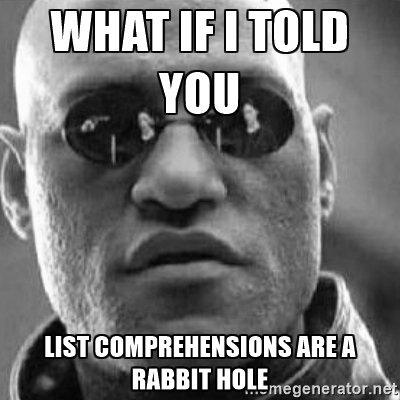
\includegraphics[width=\linewidth]{morpheus.jpg}
  \caption{Using the search term "list comprehension" on Google can open up a secret programming challenge named "foobar".  Pass the first three levels and get an interview with Google.}
  \label{fig:marginfig}
\end{marginfigure}
\begin{abstract}
\noindent
This is an introduction to list comprehensions in Python.  List comprehensions use a concise syntax,  which closely mimics mathematical notation, and provide a natural way of constructing lists.  They are easy to read and allow lists to be constructed, on the fly, without requiring multiple lines of code.    We will learn the following: 
\begin{itemize}
\item the syntax of list comprehensions
\item how to write list comprehensions
 \item example applications of list comprehensions
 \end{itemize} \end{abstract}

\normalsize

%this generates 1cm of vertical space

\section{Mathematical Notation }
The list $L$ below is described using "set builder" notation. 
\marginnote[10pt]{
\begin{center}{\large$x$ is an element of}
\Large $$x\in \mathbb{N}$$
{\large the set of natural numbers}
 $$\mathbb{N}=\{ 0,1,2,3,4...\}$$
 \end{center}}
$$L=\{\,\underbrace{\sqrt{x}}_{\color{Blue}{\text{output}}}\mid \underbrace{x}_{\color{Blue}{\text{variable}}} \in \underbrace{\mathbb{N}}_{\color{Blue}{\text{input set}}},\ \underbrace{x^2<25}_{\color{Blue}{\text{condition}}}\,\}$$

$L$ is the set of $\sqrt{x}$ \textbf{for} $x$ in the set of natural numbers $\mathbb{N}$ \textbf{if} $x^2<25$.

$$L=\{\ 0,\sqrt{1} ,\sqrt{2},\sqrt{3},\sqrt{4}\}$$

\section{In Python}

\marginnote[0pt]{
}

\begin{marginfigure}[0 pt]%
\center
  
\includegraphics[width=0.63\linewidth]{sugar.jpg}
  \caption{In computer science, \textit{\textbf{syntactic sugar} } is syntax within a programming language that is designed to make things easier to read or to express. It makes the language "sweeter" for human use: things can be expressed more clearly, more concisely, or in an alternative style that some may prefer.}
  \label{fig:marginfig}
\end{marginfigure}

We construct the set in Python, using list comprehension, as follows. 
%
% Default to the notebook output style

    


% Inherit from the specified cell style.




    
\documentclass[11pt]{article}

    
    
    \usepackage[T1]{fontenc}
    % Nicer default font than Computer Modern for most use cases
    \usepackage{palatino}

    % Basic figure setup, for now with no caption control since it's done
    % automatically by Pandoc (which extracts ![](path) syntax from Markdown).
    \usepackage{graphicx}
    % We will generate all images so they have a width \maxwidth. This means
    % that they will get their normal width if they fit onto the page, but
    % are scaled down if they would overflow the margins.
    \makeatletter
    \def\maxwidth{\ifdim\Gin@nat@width>\linewidth\linewidth
    \else\Gin@nat@width\fi}
    \makeatother
    \let\Oldincludegraphics\includegraphics
    % Set max figure width to be 80% of text width, for now hardcoded.
    \renewcommand{\includegraphics}[1]{\Oldincludegraphics[width=.8\maxwidth]{#1}}
    % Ensure that by default, figures have no caption (until we provide a
    % proper Figure object with a Caption API and a way to capture that
    % in the conversion process - todo).
    \usepackage{caption}
    \DeclareCaptionLabelFormat{nolabel}{}
    \captionsetup{labelformat=nolabel}

    \usepackage{adjustbox} % Used to constrain images to a maximum size 
    \usepackage{xcolor} % Allow colors to be defined
    \usepackage{enumerate} % Needed for markdown enumerations to work
    \usepackage{geometry} % Used to adjust the document margins
    \usepackage{amsmath} % Equations
    \usepackage{amssymb} % Equations
    \usepackage{textcomp} % defines textquotesingle
    % Hack from http://tex.stackexchange.com/a/47451/13684:
    \AtBeginDocument{%
        \def\PYZsq{\textquotesingle}% Upright quotes in Pygmentized code
    }
    \usepackage{upquote} % Upright quotes for verbatim code
    \usepackage{eurosym} % defines \euro
    \usepackage[mathletters]{ucs} % Extended unicode (utf-8) support
    \usepackage[utf8x]{inputenc} % Allow utf-8 characters in the tex document
    \usepackage{fancyvrb} % verbatim replacement that allows latex
    \usepackage{grffile} % extends the file name processing of package graphics 
                         % to support a larger range 
    % The hyperref package gives us a pdf with properly built
    % internal navigation ('pdf bookmarks' for the table of contents,
    % internal cross-reference links, web links for URLs, etc.)
    \usepackage{hyperref}
    \usepackage{longtable} % longtable support required by pandoc >1.10
    \usepackage{booktabs}  % table support for pandoc > 1.12.2
    \usepackage[normalem]{ulem} % ulem is needed to support strikethroughs (\sout)
                                % normalem makes italics be italics, not underlines
    

    
    
    % Colors for the hyperref package
    \definecolor{urlcolor}{rgb}{0,.145,.698}
    \definecolor{linkcolor}{rgb}{.71,0.21,0.01}
    \definecolor{citecolor}{rgb}{.12,.54,.11}

    % ANSI colors
    \definecolor{ansi-black}{HTML}{3E424D}
    \definecolor{ansi-black-intense}{HTML}{282C36}
    \definecolor{ansi-red}{HTML}{E75C58}
    \definecolor{ansi-red-intense}{HTML}{B22B31}
    \definecolor{ansi-green}{HTML}{00A250}
    \definecolor{ansi-green-intense}{HTML}{007427}
    \definecolor{ansi-yellow}{HTML}{DDB62B}
    \definecolor{ansi-yellow-intense}{HTML}{B27D12}
    \definecolor{ansi-blue}{HTML}{208FFB}
    \definecolor{ansi-blue-intense}{HTML}{0065CA}
    \definecolor{ansi-magenta}{HTML}{D160C4}
    \definecolor{ansi-magenta-intense}{HTML}{A03196}
    \definecolor{ansi-cyan}{HTML}{60C6C8}
    \definecolor{ansi-cyan-intense}{HTML}{258F8F}
    \definecolor{ansi-white}{HTML}{C5C1B4}
    \definecolor{ansi-white-intense}{HTML}{A1A6B2}

    % commands and environments needed by pandoc snippets
    % extracted from the output of `pandoc -s`
    \providecommand{\tightlist}{%
      \setlength{\itemsep}{0pt}\setlength{\parskip}{0pt}}
    \DefineVerbatimEnvironment{Highlighting}{Verbatim}{commandchars=\\\{\}}
    % Add ',fontsize=\small' for more characters per line
    \newenvironment{Shaded}{}{}
    \newcommand{\KeywordTok}[1]{\textcolor[rgb]{0.00,0.44,0.13}{\textbf{{#1}}}}
    \newcommand{\DataTypeTok}[1]{\textcolor[rgb]{0.56,0.13,0.00}{{#1}}}
    \newcommand{\DecValTok}[1]{\textcolor[rgb]{0.25,0.63,0.44}{{#1}}}
    \newcommand{\BaseNTok}[1]{\textcolor[rgb]{0.25,0.63,0.44}{{#1}}}
    \newcommand{\FloatTok}[1]{\textcolor[rgb]{0.25,0.63,0.44}{{#1}}}
    \newcommand{\CharTok}[1]{\textcolor[rgb]{0.25,0.44,0.63}{{#1}}}
    \newcommand{\StringTok}[1]{\textcolor[rgb]{0.25,0.44,0.63}{{#1}}}
    \newcommand{\CommentTok}[1]{\textcolor[rgb]{0.38,0.63,0.69}{\textit{{#1}}}}
    \newcommand{\OtherTok}[1]{\textcolor[rgb]{0.00,0.44,0.13}{{#1}}}
    \newcommand{\AlertTok}[1]{\textcolor[rgb]{1.00,0.00,0.00}{\textbf{{#1}}}}
    \newcommand{\FunctionTok}[1]{\textcolor[rgb]{0.02,0.16,0.49}{{#1}}}
    \newcommand{\RegionMarkerTok}[1]{{#1}}
    \newcommand{\ErrorTok}[1]{\textcolor[rgb]{1.00,0.00,0.00}{\textbf{{#1}}}}
    \newcommand{\NormalTok}[1]{{#1}}
    
    % Additional commands for more recent versions of Pandoc
    \newcommand{\ConstantTok}[1]{\textcolor[rgb]{0.53,0.00,0.00}{{#1}}}
    \newcommand{\SpecialCharTok}[1]{\textcolor[rgb]{0.25,0.44,0.63}{{#1}}}
    \newcommand{\VerbatimStringTok}[1]{\textcolor[rgb]{0.25,0.44,0.63}{{#1}}}
    \newcommand{\SpecialStringTok}[1]{\textcolor[rgb]{0.73,0.40,0.53}{{#1}}}
    \newcommand{\ImportTok}[1]{{#1}}
    \newcommand{\DocumentationTok}[1]{\textcolor[rgb]{0.73,0.13,0.13}{\textit{{#1}}}}
    \newcommand{\AnnotationTok}[1]{\textcolor[rgb]{0.38,0.63,0.69}{\textbf{\textit{{#1}}}}}
    \newcommand{\CommentVarTok}[1]{\textcolor[rgb]{0.38,0.63,0.69}{\textbf{\textit{{#1}}}}}
    \newcommand{\VariableTok}[1]{\textcolor[rgb]{0.10,0.09,0.49}{{#1}}}
    \newcommand{\ControlFlowTok}[1]{\textcolor[rgb]{0.00,0.44,0.13}{\textbf{{#1}}}}
    \newcommand{\OperatorTok}[1]{\textcolor[rgb]{0.40,0.40,0.40}{{#1}}}
    \newcommand{\BuiltInTok}[1]{{#1}}
    \newcommand{\ExtensionTok}[1]{{#1}}
    \newcommand{\PreprocessorTok}[1]{\textcolor[rgb]{0.74,0.48,0.00}{{#1}}}
    \newcommand{\AttributeTok}[1]{\textcolor[rgb]{0.49,0.56,0.16}{{#1}}}
    \newcommand{\InformationTok}[1]{\textcolor[rgb]{0.38,0.63,0.69}{\textbf{\textit{{#1}}}}}
    \newcommand{\WarningTok}[1]{\textcolor[rgb]{0.38,0.63,0.69}{\textbf{\textit{{#1}}}}}
    
    
    % Define a nice break command that doesn't care if a line doesn't already
    % exist.
    \def\br{\hspace*{\fill} \\* }
    % Math Jax compatability definitions
    \def\gt{>}
    \def\lt{<}
    % Document parameters
    \title{Untitled}
    
    
    

    % Pygments definitions
    
\makeatletter
\def\PY@reset{\let\PY@it=\relax \let\PY@bf=\relax%
    \let\PY@ul=\relax \let\PY@tc=\relax%
    \let\PY@bc=\relax \let\PY@ff=\relax}
\def\PY@tok#1{\csname PY@tok@#1\endcsname}
\def\PY@toks#1+{\ifx\relax#1\empty\else%
    \PY@tok{#1}\expandafter\PY@toks\fi}
\def\PY@do#1{\PY@bc{\PY@tc{\PY@ul{%
    \PY@it{\PY@bf{\PY@ff{#1}}}}}}}
\def\PY#1#2{\PY@reset\PY@toks#1+\relax+\PY@do{#2}}

\expandafter\def\csname PY@tok@na\endcsname{\def\PY@tc##1{\textcolor[rgb]{0.49,0.56,0.16}{##1}}}
\expandafter\def\csname PY@tok@ss\endcsname{\def\PY@tc##1{\textcolor[rgb]{0.10,0.09,0.49}{##1}}}
\expandafter\def\csname PY@tok@bp\endcsname{\def\PY@tc##1{\textcolor[rgb]{0.00,0.50,0.00}{##1}}}
\expandafter\def\csname PY@tok@c1\endcsname{\let\PY@it=\textit\def\PY@tc##1{\textcolor[rgb]{0.25,0.50,0.50}{##1}}}
\expandafter\def\csname PY@tok@gd\endcsname{\def\PY@tc##1{\textcolor[rgb]{0.63,0.00,0.00}{##1}}}
\expandafter\def\csname PY@tok@sc\endcsname{\def\PY@tc##1{\textcolor[rgb]{0.73,0.13,0.13}{##1}}}
\expandafter\def\csname PY@tok@sb\endcsname{\def\PY@tc##1{\textcolor[rgb]{0.73,0.13,0.13}{##1}}}
\expandafter\def\csname PY@tok@gr\endcsname{\def\PY@tc##1{\textcolor[rgb]{1.00,0.00,0.00}{##1}}}
\expandafter\def\csname PY@tok@cp\endcsname{\def\PY@tc##1{\textcolor[rgb]{0.74,0.48,0.00}{##1}}}
\expandafter\def\csname PY@tok@ge\endcsname{\let\PY@it=\textit}
\expandafter\def\csname PY@tok@s\endcsname{\def\PY@tc##1{\textcolor[rgb]{0.73,0.13,0.13}{##1}}}
\expandafter\def\csname PY@tok@ne\endcsname{\let\PY@bf=\textbf\def\PY@tc##1{\textcolor[rgb]{0.82,0.25,0.23}{##1}}}
\expandafter\def\csname PY@tok@mo\endcsname{\def\PY@tc##1{\textcolor[rgb]{0.40,0.40,0.40}{##1}}}
\expandafter\def\csname PY@tok@kp\endcsname{\def\PY@tc##1{\textcolor[rgb]{0.00,0.50,0.00}{##1}}}
\expandafter\def\csname PY@tok@kr\endcsname{\let\PY@bf=\textbf\def\PY@tc##1{\textcolor[rgb]{0.00,0.50,0.00}{##1}}}
\expandafter\def\csname PY@tok@sr\endcsname{\def\PY@tc##1{\textcolor[rgb]{0.73,0.40,0.53}{##1}}}
\expandafter\def\csname PY@tok@kn\endcsname{\let\PY@bf=\textbf\def\PY@tc##1{\textcolor[rgb]{0.00,0.50,0.00}{##1}}}
\expandafter\def\csname PY@tok@nf\endcsname{\def\PY@tc##1{\textcolor[rgb]{0.00,0.00,1.00}{##1}}}
\expandafter\def\csname PY@tok@ch\endcsname{\let\PY@it=\textit\def\PY@tc##1{\textcolor[rgb]{0.25,0.50,0.50}{##1}}}
\expandafter\def\csname PY@tok@ni\endcsname{\let\PY@bf=\textbf\def\PY@tc##1{\textcolor[rgb]{0.60,0.60,0.60}{##1}}}
\expandafter\def\csname PY@tok@ow\endcsname{\let\PY@bf=\textbf\def\PY@tc##1{\textcolor[rgb]{0.67,0.13,1.00}{##1}}}
\expandafter\def\csname PY@tok@nd\endcsname{\def\PY@tc##1{\textcolor[rgb]{0.67,0.13,1.00}{##1}}}
\expandafter\def\csname PY@tok@kd\endcsname{\let\PY@bf=\textbf\def\PY@tc##1{\textcolor[rgb]{0.00,0.50,0.00}{##1}}}
\expandafter\def\csname PY@tok@gp\endcsname{\let\PY@bf=\textbf\def\PY@tc##1{\textcolor[rgb]{0.00,0.00,0.50}{##1}}}
\expandafter\def\csname PY@tok@gs\endcsname{\let\PY@bf=\textbf}
\expandafter\def\csname PY@tok@si\endcsname{\let\PY@bf=\textbf\def\PY@tc##1{\textcolor[rgb]{0.73,0.40,0.53}{##1}}}
\expandafter\def\csname PY@tok@cm\endcsname{\let\PY@it=\textit\def\PY@tc##1{\textcolor[rgb]{0.25,0.50,0.50}{##1}}}
\expandafter\def\csname PY@tok@nl\endcsname{\def\PY@tc##1{\textcolor[rgb]{0.63,0.63,0.00}{##1}}}
\expandafter\def\csname PY@tok@kt\endcsname{\def\PY@tc##1{\textcolor[rgb]{0.69,0.00,0.25}{##1}}}
\expandafter\def\csname PY@tok@se\endcsname{\let\PY@bf=\textbf\def\PY@tc##1{\textcolor[rgb]{0.73,0.40,0.13}{##1}}}
\expandafter\def\csname PY@tok@w\endcsname{\def\PY@tc##1{\textcolor[rgb]{0.73,0.73,0.73}{##1}}}
\expandafter\def\csname PY@tok@il\endcsname{\def\PY@tc##1{\textcolor[rgb]{0.40,0.40,0.40}{##1}}}
\expandafter\def\csname PY@tok@mh\endcsname{\def\PY@tc##1{\textcolor[rgb]{0.40,0.40,0.40}{##1}}}
\expandafter\def\csname PY@tok@err\endcsname{\def\PY@bc##1{\setlength{\fboxsep}{0pt}\fcolorbox[rgb]{1.00,0.00,0.00}{1,1,1}{\strut ##1}}}
\expandafter\def\csname PY@tok@sx\endcsname{\def\PY@tc##1{\textcolor[rgb]{0.00,0.50,0.00}{##1}}}
\expandafter\def\csname PY@tok@kc\endcsname{\let\PY@bf=\textbf\def\PY@tc##1{\textcolor[rgb]{0.00,0.50,0.00}{##1}}}
\expandafter\def\csname PY@tok@nt\endcsname{\let\PY@bf=\textbf\def\PY@tc##1{\textcolor[rgb]{0.00,0.50,0.00}{##1}}}
\expandafter\def\csname PY@tok@o\endcsname{\def\PY@tc##1{\textcolor[rgb]{0.40,0.40,0.40}{##1}}}
\expandafter\def\csname PY@tok@cs\endcsname{\let\PY@it=\textit\def\PY@tc##1{\textcolor[rgb]{0.25,0.50,0.50}{##1}}}
\expandafter\def\csname PY@tok@k\endcsname{\let\PY@bf=\textbf\def\PY@tc##1{\textcolor[rgb]{0.00,0.50,0.00}{##1}}}
\expandafter\def\csname PY@tok@mf\endcsname{\def\PY@tc##1{\textcolor[rgb]{0.40,0.40,0.40}{##1}}}
\expandafter\def\csname PY@tok@no\endcsname{\def\PY@tc##1{\textcolor[rgb]{0.53,0.00,0.00}{##1}}}
\expandafter\def\csname PY@tok@m\endcsname{\def\PY@tc##1{\textcolor[rgb]{0.40,0.40,0.40}{##1}}}
\expandafter\def\csname PY@tok@s1\endcsname{\def\PY@tc##1{\textcolor[rgb]{0.73,0.13,0.13}{##1}}}
\expandafter\def\csname PY@tok@cpf\endcsname{\let\PY@it=\textit\def\PY@tc##1{\textcolor[rgb]{0.25,0.50,0.50}{##1}}}
\expandafter\def\csname PY@tok@vc\endcsname{\def\PY@tc##1{\textcolor[rgb]{0.10,0.09,0.49}{##1}}}
\expandafter\def\csname PY@tok@gu\endcsname{\let\PY@bf=\textbf\def\PY@tc##1{\textcolor[rgb]{0.50,0.00,0.50}{##1}}}
\expandafter\def\csname PY@tok@vg\endcsname{\def\PY@tc##1{\textcolor[rgb]{0.10,0.09,0.49}{##1}}}
\expandafter\def\csname PY@tok@sd\endcsname{\let\PY@it=\textit\def\PY@tc##1{\textcolor[rgb]{0.73,0.13,0.13}{##1}}}
\expandafter\def\csname PY@tok@nc\endcsname{\let\PY@bf=\textbf\def\PY@tc##1{\textcolor[rgb]{0.00,0.00,1.00}{##1}}}
\expandafter\def\csname PY@tok@mb\endcsname{\def\PY@tc##1{\textcolor[rgb]{0.40,0.40,0.40}{##1}}}
\expandafter\def\csname PY@tok@go\endcsname{\def\PY@tc##1{\textcolor[rgb]{0.53,0.53,0.53}{##1}}}
\expandafter\def\csname PY@tok@sh\endcsname{\def\PY@tc##1{\textcolor[rgb]{0.73,0.13,0.13}{##1}}}
\expandafter\def\csname PY@tok@nn\endcsname{\let\PY@bf=\textbf\def\PY@tc##1{\textcolor[rgb]{0.00,0.00,1.00}{##1}}}
\expandafter\def\csname PY@tok@gi\endcsname{\def\PY@tc##1{\textcolor[rgb]{0.00,0.63,0.00}{##1}}}
\expandafter\def\csname PY@tok@vi\endcsname{\def\PY@tc##1{\textcolor[rgb]{0.10,0.09,0.49}{##1}}}
\expandafter\def\csname PY@tok@mi\endcsname{\def\PY@tc##1{\textcolor[rgb]{0.40,0.40,0.40}{##1}}}
\expandafter\def\csname PY@tok@nv\endcsname{\def\PY@tc##1{\textcolor[rgb]{0.10,0.09,0.49}{##1}}}
\expandafter\def\csname PY@tok@gh\endcsname{\let\PY@bf=\textbf\def\PY@tc##1{\textcolor[rgb]{0.00,0.00,0.50}{##1}}}
\expandafter\def\csname PY@tok@c\endcsname{\let\PY@it=\textit\def\PY@tc##1{\textcolor[rgb]{0.25,0.50,0.50}{##1}}}
\expandafter\def\csname PY@tok@nb\endcsname{\def\PY@tc##1{\textcolor[rgb]{0.00,0.50,0.00}{##1}}}
\expandafter\def\csname PY@tok@gt\endcsname{\def\PY@tc##1{\textcolor[rgb]{0.00,0.27,0.87}{##1}}}
\expandafter\def\csname PY@tok@s2\endcsname{\def\PY@tc##1{\textcolor[rgb]{0.73,0.13,0.13}{##1}}}

\def\PYZbs{\char`\\}
\def\PYZus{\char`\_}
\def\PYZob{\char`\{}
\def\PYZcb{\char`\}}
\def\PYZca{\char`\^}
\def\PYZam{\char`\&}
\def\PYZlt{\char`\<}
\def\PYZgt{\char`\>}
\def\PYZsh{\char`\#}
\def\PYZpc{\char`\%}
\def\PYZdl{\char`\$}
\def\PYZhy{\char`\-}
\def\PYZsq{\char`\'}
\def\PYZdq{\char`\"}
\def\PYZti{\char`\~}
% for compatibility with earlier versions
\def\PYZat{@}
\def\PYZlb{[}
\def\PYZrb{]}
\makeatother


    % Exact colors from NB
    \definecolor{incolor}{rgb}{0.0, 0.0, 0.5}
    \definecolor{outcolor}{rgb}{0.545, 0.0, 0.0}



    
    % Prevent overflowing lines due to hard-to-break entities
    \sloppy 
    % Setup hyperref package
    \hypersetup{
      breaklinks=true,  % so long urls are correctly broken across lines
      colorlinks=true,
      urlcolor=urlcolor,
      linkcolor=linkcolor,
      citecolor=citecolor,
      }
    % Slightly bigger margins than the latex defaults
    
    \geometry{verbose,tmargin=1in,bmargin=1in,lmargin=1in,rmargin=1in}
    
    

    \begin{document}
    
    
  
    
    

    \small
    \begin{Verbatim}[commandchars=\\\{\}]
{\color{incolor}In [{\color{incolor}1}]:} \PY{p}{[}\PY{n}{x}\PY{o}{*}\PY{o}{*}\PY{l+m+mf}{0.5} \PY{k}{for} \PY{n}{x} \PY{o+ow}{in} \PY{n+nb}{range}\PY{p}{(}\PY{l+m+mi}{100}\PY{p}{)} \PY{k}{if} \PY{n}{x}\PY{o}{*}\PY{o}{*}\PY{l+m+mi}{2}\PY{o}{\PYZlt{}}\PY{l+m+mi}{25}\PY{p}{]}
\end{Verbatim}

            \begin{Verbatim}[commandchars=\\\{\}]
{\color{outcolor}Out[{\color{outcolor}1}]:} [0.0, 1.0, 1.4142135623730951, 1.7320508075688772, 2.0]
\end{Verbatim}
        
  


    % Add a bibliography block to the postdoc
    
    
    
    \end{document}


 \begin{shaded}
    \begin{Verbatim}[fontsize=\small,commandchars=\\\{\}] 
{\color{incolor}In [{\color{incolor}1}]:} \PY{p}{[}\PY{n}{x}\PY{o}{*}\PY{o}{*}\PY{l+m+mf}{0.5} \PY{k}{for} \PY{n}{x} \PY{o+ow}{in} \PY{n+nb}{range}\PY{p}{(}\PY{l+m+mi}{100}\PY{p}{)} \PY{k}{if} \PY{n}{x}\PY{o}{*}\PY{o}{*}\PY{l+m+mi}{2}\PY{o}{\PYZlt{}}\PY{l+m+mi}{25}\PY{p}{]}
\end{Verbatim}
 \begin{Verbatim}[fontsize=\small,commandchars=\\\{\}]
{\color{outcolor}Out[{\color{outcolor}1}]:} [0.0, 1.0, 1.4142135623730951, 1.7320508075688772, 2.0]
\end{Verbatim}
\end{shaded}

\noindent This set can be constructed using a conditional statement inside a for loop. 

\begin{shaded}
 \begin{Verbatim}[fontsize=\small,commandchars=\\\{\}]
{\color{incolor}In [{\color{incolor}2}]:} \PY{n}{L}\PY{o}{=}\PY{p}{[}\PY{p}{]}
        \PY{k}{for} \PY{n}{x} \PY{o+ow}{in} \PY{n+nb}{range}\PY{p}{(}\PY{l+m+mi}{100}\PY{p}{)}\PY{p}{:}
            \PY{k}{if} \PY{n}{x}\PY{o}{*}\PY{o}{*}\PY{l+m+mi}{2}\PY{o}{\PYZlt{}}\PY{l+m+mi}{25}\PY{p}{:}
                \PY{n}{L}\PY{o}{.}\PY{n}{append}\PY{p}{(}\PY{n}{x}\PY{o}{*}\PY{o}{*}\PY{l+m+mf}{0.5}\PY{p}{)}
        \PY{n}{L}
\end{Verbatim}

            \begin{Verbatim}[fontsize=\small,commandchars=\\\{\}]
{\color{outcolor}Out[{\color{outcolor}2}]:} [0.0, 1.0, 1.4142135623730951, 1.7320508075688772, 2.0]
\end{Verbatim}

\end{shaded}

\normalsize
\noindent This set can also be constructed using \textbf{filter()}, \textbf{map()} and \textbf{lambda} magic.
 
\begin{shaded}
  \begin{Verbatim}[fontsize=\small,commandchars=\\\{\}]
{\color{incolor}In [{\color{incolor}3}]:} \PY{n}{M}\PY{o}{=}\PY{n+nb}{list}\PY{p}{(}\PY{n+nb}{filter}\PY{p}{(}\PY{k}{lambda} \PY{n}{x}\PY{p}{:} \PY{n}{x}\PY{o}{*}\PY{o}{*}\PY{l+m+mi}{2} \PY{o}{\PYZlt{}} \PY{l+m+mi}{25}\PY{p}{,} \PY{n+nb}{range}\PY{p}{(}\PY{l+m+mi}{100}\PY{p}{)}\PY{p}{)}\PY{p}{)}
        \PY{n}{L}\PY{o}{=}\PY{n+nb}{list}\PY{p}{(}\PY{n+nb}{map}\PY{p}{(}\PY{k}{lambda} \PY{n}{x}\PY{p}{:} \PY{n}{x}\PY{o}{*}\PY{o}{*}\PY{l+m+mf}{0.5}\PY{p}{,} \PY{n}{M}\PY{p}{)}\PY{p}{)}
        \PY{n}{L}
\end{Verbatim}

            \begin{Verbatim}[fontsize=\small,commandchars=\\\{\}]
{\color{outcolor}Out[{\color{outcolor}3}]:} [0.0, 1.0, 1.4142135623730951, 1.7320508075688772, 2.0]
\end{Verbatim}
\end{shaded}






\begin{marginfigure}[-130 pt]%
\center
  \includegraphics[width=0.63\linewidth]{lambda_map.png}
  \caption{List comprehensions are a complete substitute for the lambda function as well as the functions map(), filter() and reduce(). }
  \label{fig:marginfig}
\end{marginfigure}




\marginnote[30pt]{\newcommand{\pythagwidth}{1.8cm}
\newcommand{\pythagheight}{1.2cm}

$$\begin{tikzpicture}

  \coordinate [label={below right:$ $}] (A) at (0, 0);
  \coordinate [label={above right:$ $}] (B) at (0, \pythagheight);
  \coordinate [label={below left:$ $}] (C) at (-\pythagwidth, 0);

  \coordinate (D1) at (-\pythagheight, \pythagheight + \pythagwidth);
  \coordinate (D2) at (-\pythagheight - \pythagwidth, \pythagwidth);

  \draw [very thick] (A) -- (C) -- (B) -- (A);

  \newcommand{\ranglesize}{0.3cm}
  \draw (A) -- ++ (0, \ranglesize) -- ++ (-\ranglesize, 0) -- ++ (0, -\ranglesize);

  \draw [dashed] (A) -- node [below] {$x$} ++ (-\pythagwidth, 0)
            -- node [right] {$ $} ++ (0, -\pythagwidth)
            -- node [above] {$ $} ++ (\pythagwidth, 0)
            -- node [left] {$ $} ++ (0, \pythagwidth);

  \draw [dashed] (A) -- node [right] {$y$} ++ (0, \pythagheight)
            -- node [below] {$ $} ++ (\pythagheight, 0)
            -- node [left] {$ $} ++ (0, -\pythagheight)
            -- node [above] {$ $} ++ (-\pythagheight, 0);

  \draw [dashed] (C) -- node [above left] {$z$} (B)
                     -- node [below left] {$ $} (D1)
                     -- node [below right] {$ $} (D2)
                     -- node [above right] {$ $} (C);

\end{tikzpicture}$$
Pythagorean triples describe the three integer side lengths of a right triangle.  The name is derived from the Pythagorean theorem.
$$x^2+y^2=z^2$$}

\section{Example Zero: Pythagorean Triples}
This example shows how to construct Pythagorean triples.  It uses three indices, $x,y$ and $z$ and filters for the condition $x^2+y^2=z^2$.

\begin{shaded}

       \begin{Verbatim}[fontsize=\small,commandchars=\\\{\}]
{\color{incolor}In [{\color{incolor}4}]:} \PY{n}{P}\PY{o}{=}\PY{p}{[}\PY{p}{[}\PY{n}{x}\PY{p}{,}\PY{n}{y}\PY{p}{,}\PY{n}{z}\PY{p}{]} \PY{k}{for} \PY{n}{x} \PY{o+ow}{in} \PY{n+nb}{range}\PY{p}{(}\PY{l+m+mi}{1}\PY{p}{,}\PY{l+m+mi}{26}\PY{p}{)} \PYZbs{}
            \PY{k}{for} \PY{n}{y} \PY{o+ow}{in} \PY{n+nb}{range}\PY{p}{(}\PY{n}{x}\PY{p}{,}\PY{l+m+mi}{26}\PY{p}{)} \PYZbs{}
            \PY{k}{for} \PY{n}{z} \PY{o+ow}{in} \PY{n+nb}{range}\PY{p}{(}\PY{n}{y}\PY{p}{,}\PY{l+m+mi}{26}\PY{p}{)} \PY{k}{if} \PY{n}{x}\PY{o}{*}\PY{o}{*}\PY{l+m+mi}{2} \PY{o}{+} \PY{n}{y}\PY{o}{*}\PY{o}{*}\PY{l+m+mi}{2} \PY{o}{==} \PY{n}{z}\PY{o}{*}\PY{o}{*}\PY{l+m+mi}{2}\PY{p}{]}
        \PY{n}{P}
\end{Verbatim}


            \begin{Verbatim}[fontsize=\small,commandchars=\\\{\}]
{\color{outcolor}Out[{\color{outcolor}4}]:} [[3, 4, 5],
          [5, 12, 13],
          [6, 8, 10],
          [7, 24, 25],
          [8, 15, 17],
          [9, 12, 15],
          [12, 16, 20],
          [15, 20, 25]]
\end{Verbatim}
\end{shaded}

\section{Example One: 1-D Centroid Analysis}
\marginnote[60pt]{
Given a list $a$ the sum of the list is $a_0$.
$$a_0=\int  a(x)\ dx$$
The position weighted sum of the list is $a_X$.
$$a_X=\int  a(x)\ x\ dx$$
The center of mass, or centroid, of $a$ is $\bar{a}_x$.
$$\bar{a}_x=\frac{a_X}{a_0}$$}

Here we use list comprehension to succinctly compute average position of a 1-D distribution.  We define a list representing the position of each cell, $X$.  
 \begin{shaded}   
     \begin{Verbatim}[fontsize=\small,commandchars=\\\{\}]
{\color{incolor}In [{\color{incolor}5}]:} \PY{n}{mx}\PY{o}{=}\PY{l+m+mi}{5}
        \PY{n}{X}\PY{o}{=}\PY{p}{[}\PY{n}{x}\PY{o}{/}\PY{p}{(}\PY{n}{mx}\PY{o}{\PYZhy{}}\PY{l+m+mi}{1}\PY{p}{)} \PY{k}{for} \PY{n}{x} \PY{o+ow}{in} \PY{n+nb}{range}\PY{p}{(}\PY{n}{mx}\PY{p}{)}\PY{p}{]}
        \PY{n}{X}
\end{Verbatim}

            \begin{Verbatim}[fontsize=\small,commandchars=\\\{\}]
{\color{outcolor}Out[{\color{outcolor}5}]:} [0.0, 0.25, 0.5, 0.75, 1.0]
\end{Verbatim}
        
    \begin{Verbatim}[fontsize=\small,commandchars=\\\{\}]
{\color{incolor}In [{\color{incolor}6}]:} \PY{n}{a}\PY{o}{=}\PY{p}{[}\PY{l+m+mi}{4}\PY{p}{,}\PY{l+m+mi}{5}\PY{p}{,}\PY{l+m+mi}{0}\PY{p}{,}\PY{l+m+mi}{0}\PY{p}{,}\PY{l+m+mi}{1}\PY{p}{]}
        \PY{n}{a0}\PY{o}{=}\PY{n+nb}{sum}\PY{p}{(}\PY{n}{a}\PY{p}{)}
        \PY{n}{aX}\PY{o}{=}\PY{n+nb}{sum}\PY{p}{(}\PY{p}{[}\PY{n}{X}\PY{p}{[}\PY{n}{i}\PY{p}{]}\PY{o}{*}\PY{n}{a}\PY{p}{[}\PY{n}{i}\PY{p}{]} \PY{k}{for} \PY{n}{i} \PY{o+ow}{in} \PY{n+nb}{range}\PY{p}{(}\PY{n}{mx}\PY{p}{)}\PY{p}{]}\PY{p}{)}
        \PY{n}{aX}\PY{o}{/}\PY{n}{a0}
\end{Verbatim}

            \begin{Verbatim}[fontsize=\small, commandchars=\\\{\}]
{\color{outcolor}Out[{\color{outcolor}6}]:} 0.225
\end{Verbatim}
\end{shaded}
    
\section{Example Two: 2-D Centroid Analysis}  
\marginnote[-30pt]{ \center \includegraphics[width=\linewidth]{centroid.png}}
In this example we apply centroid analysis in two dimensions.  As in the previous example we construct the lists $X$ and $Y$.  These are now 2-D lists of lists.
 \marginnote[10pt]{
Given a 2-D list $A$ the sum of the list is $A_0$.
$$A_0=\int  \int A(x,y)\ dx \ dy$$
\vspace{1cm}

$A_X$ is the x-position weighted sum of $A$.
$$A_X=\int  \int A(x,y)\ x\ dx \ dy$$
\vspace{1cm}

$A_Y$ is the y-position weighted sum of $A$.
$$A_Y=\int  \int A(x,y)\ y\ dx \ dy$$
\vspace{1cm}

The 2-D centroid of $A$ is $\left(\frac{A_X}{A_0},\frac{A_Y}{A_0}\right)$.}
  \begin{shaded}
    \begin{Verbatim}[fontsize=\small,commandchars=\\\{\}]
{\color{incolor}In [{\color{incolor}7}]:} \PY{n}{mx}\PY{o}{=}\PY{l+m+mi}{5}
        \PY{n}{my}\PY{o}{=}\PY{l+m+mi}{6}
        \PY{n}{X}\PY{o}{=}\PY{p}{[}\PY{p}{[}\PY{n}{x}\PY{o}{/}\PY{p}{(}\PY{n}{mx}\PY{o}{\PYZhy{}}\PY{l+m+mi}{1}\PY{p}{)} \PY{k}{for} \PY{n}{x} \PY{o+ow}{in} \PY{n+nb}{range}\PY{p}{(}\PY{n}{mx}\PY{p}{)}\PY{p}{]} \PY{k}{for} \PY{n}{y} \PY{o+ow}{in} \PY{n+nb}{range}\PY{p}{(}\PY{n}{my}\PY{p}{)} \PY{p}{]}
        \PY{n}{X}
\end{Verbatim}

            \begin{Verbatim}[fontsize=\small,commandchars=\\\{\}]
{\color{outcolor}Out[{\color{outcolor}7}]:} [[0.0, 0.25, 0.5, 0.75, 1.0],
         [0.0, 0.25, 0.5, 0.75, 1.0],
         [0.0, 0.25, 0.5, 0.75, 1.0],
         [0.0, 0.25, 0.5, 0.75, 1.0],
         [0.0, 0.25, 0.5, 0.75, 1.0],
         [0.0, 0.25, 0.5, 0.75, 1.0]]
\end{Verbatim}
        
    \begin{Verbatim}[fontsize=\small,commandchars=\\\{\}]
{\color{incolor}In [{\color{incolor}8}]:} \PY{n}{Y}\PY{o}{=}\PY{p}{[}\PY{p}{[}\PY{n}{y}\PY{o}{/}\PY{p}{(}\PY{n}{my}\PY{o}{\PYZhy{}}\PY{l+m+mi}{1}\PY{p}{)} \PY{k}{for} \PY{n}{x} \PY{o+ow}{in} \PY{n+nb}{range}\PY{p}{(}\PY{n}{mx}\PY{p}{)}\PY{p}{]} \PY{k}{for} \PY{n}{y} \PY{o+ow}{in} \PY{n+nb}{range}\PY{p}{(}\PY{n}{my}\PY{p}{)} \PY{p}{]}
        \PY{n}{Y}
\end{Verbatim}

            \begin{Verbatim}[fontsize=\small,commandchars=\\\{\}]
{\color{outcolor}Out[{\color{outcolor}8}]:} [[0.0, 0.0, 0.0, 0.0, 0.0],
         [0.2, 0.2, 0.2, 0.2, 0.2],
         [0.4, 0.4, 0.4, 0.4, 0.4],
         [0.6, 0.6, 0.6, 0.6, 0.6],
         [0.8, 0.8, 0.8, 0.8, 0.8],
         [1.0, 1.0, 1.0, 1.0, 1.0]]
          \end{Verbatim}
          \end{shaded}
          
          
    \noindent\rule{16cm}{1pt}
          
   \begin{fullwidth}  
      
  % \begin{framed}       
           \begin{Verbatim}[fontsize=\small, commandchars=\\\{\}]
\PY{k}{def} \PY{n+nf}{centroids}\PY{p}{(}\PY{n}{A}\PY{p}{)}\PY{p}{:}
    \PY{n}{my}\PY{o}{=}\PY{n+nb}{len}\PY{p}{(}\PY{n}{A}\PY{p}{)}
    \PY{n}{mx}\PY{o}{=}\PY{n+nb}{len}\PY{p}{(}\PY{n}{A}\PY{p}{[}\PY{l+m+mi}{0}\PY{p}{]}\PY{p}{)}
    \PY{n}{A0}\PY{o}{=}\PY{n+nb}{sum}\PY{p}{(}\PY{p}{[}\PY{n+nb}{sum}\PY{p}{(}\PY{p}{[}\PY{n}{A}\PY{p}{[}\PY{n}{i}\PY{p}{]}\PY{p}{[}\PY{n}{j}\PY{p}{]} \PY{k}{for} \PY{n}{i} \PY{o+ow}{in} \PY{n+nb}{range}\PY{p}{(}\PY{n}{my}\PY{p}{)}\PY{p}{]}\PY{p}{)} \PY{k}{for} \PY{n}{j} \PY{o+ow}{in} \PY{n+nb}{range}\PY{p}{(}\PY{n}{mx}\PY{p}{)}\PY{p}{]}\PY{p}{)}
    \PY{n}{X}\PY{o}{=}\PY{p}{[}\PY{p}{[}\PY{n}{x}\PY{o}{/}\PY{p}{(}\PY{n}{mx}\PY{o}{\PYZhy{}}\PY{l+m+mi}{1}\PY{p}{)} \PY{k}{for} \PY{n}{x} \PY{o+ow}{in} \PY{n+nb}{range}\PY{p}{(}\PY{n}{mx}\PY{p}{)}\PY{p}{]} \PY{k}{for} \PY{n}{y} \PY{o+ow}{in} \PY{n+nb}{range}\PY{p}{(}\PY{n}{my}\PY{p}{)} \PY{p}{]}
    \PY{n}{Y}\PY{o}{=}\PY{p}{[}\PY{p}{[}\PY{n}{y}\PY{o}{/}\PY{p}{(}\PY{n}{my}\PY{o}{\PYZhy{}}\PY{l+m+mi}{1}\PY{p}{)} \PY{k}{for} \PY{n}{x} \PY{o+ow}{in} \PY{n+nb}{range}\PY{p}{(}\PY{n}{mx}\PY{p}{)}\PY{p}{]} \PY{k}{for} \PY{n}{y} \PY{o+ow}{in} \PY{n+nb}{range}\PY{p}{(}\PY{n}{my}\PY{p}{)} \PY{p}{]}
    \PY{n}{AX}\PY{o}{=}\PY{n+nb}{sum}\PY{p}{(}\PY{p}{[}\PY{n+nb}{sum}\PY{p}{(}\PY{p}{[}\PY{n}{A}\PY{p}{[}\PY{n}{i}\PY{p}{]}\PY{p}{[}\PY{n}{j}\PY{p}{]}\PY{o}{*}\PY{n}{X}\PY{p}{[}\PY{n}{i}\PY{p}{]}\PY{p}{[}\PY{n}{j}\PY{p}{]} \PY{k}{for} \PY{n}{i} \PY{o+ow}{in} \PY{n+nb}{range}\PY{p}{(}\PY{n}{my}\PY{p}{)}\PY{p}{]}\PY{p}{)} \PY{k}{for} \PY{n}{j} \PY{o+ow}{in} \PY{n+nb}{range}\PY{p}{(}\PY{n}{mx}\PY{p}{)}\PY{p}{]}\PY{p}{)}
    \PY{n}{AY}\PY{o}{=}\PY{n+nb}{sum}\PY{p}{(}\PY{p}{[}\PY{n+nb}{sum}\PY{p}{(}\PY{p}{[}\PY{n}{A}\PY{p}{[}\PY{n}{i}\PY{p}{]}\PY{p}{[}\PY{n}{j}\PY{p}{]}\PY{o}{*}\PY{n}{Y}\PY{p}{[}\PY{n}{i}\PY{p}{]}\PY{p}{[}\PY{n}{j}\PY{p}{]} \PY{k}{for} \PY{n}{i} \PY{o+ow}{in} \PY{n+nb}{range}\PY{p}{(}\PY{n}{my}\PY{p}{)}\PY{p}{]}\PY{p}{)} \PY{k}{for} \PY{n}{j} \PY{o+ow}{in} \PY{n+nb}{range}\PY{p}{(}\PY{n}{mx}\PY{p}{)}\PY{p}{]}\PY{p}{)}
    \PY{n}{Ax}\PY{o}{=}\PY{n}{AX}\PY{o}{/}\PY{n}{A0}
    \PY{n}{Ay}\PY{o}{=}\PY{n}{AY}\PY{o}{/}\PY{n}{A0}
    \PY{k}{return} \PY{p}{(}\PY{n}{Ax}\PY{p}{,}\PY{n}{Ay}\PY{p}{)}
\end{Verbatim}
%\end{framed}
\end{fullwidth}
   \noindent\rule{16cm}{1pt}

\begin{shaded}
 \begin{Verbatim}[fontsize=\small,commandchars=\\\{\}]
{\color{incolor}In [{\color{incolor}9}]:} \PY{n}{centroids}\PY{p}{(}\PY{n}{P}\PY{p}{)}
\end{Verbatim}

            \begin{Verbatim}[fontsize=\small,commandchars=\\\{\}]
{\color{outcolor}Out[{\color{outcolor}9}]:} (0.6062091503267973, 0.6041083099906629)
\end{Verbatim}
\end{shaded}

\section{Example Three: Natural Language Processing }
\marginnote[20pt]{\small In this final example we use list comprehension to process a word frequency histogram.  The dictionary \texttt{\textbf{histo}} is constructed to record the frequency of each word in the example text.\\
The bag-of-words model is a simplifying representation used in natural language processing and information retrieval.   In practice, the Bag-of-words model is mainly used as a tool of feature generation. After transforming the text into a "bag of words", we can calculate various measures to characterize the text. The most common type of characteristics, or features calculated from the Bag-of-words model is term frequency, namely, the number of times a term appears in the text.} 
\marginnote[10pt]{ \center 
\includegraphics[width=\linewidth]{bag.jpg}}
\marginnote[20pt]{\small We process \texttt{\textbf{histo}} first by creating a list of tuples for repeated words.  Restricting the list to repeated words means we filter for frequencies greater than 1.  The tuples have the frequency first and the word second.  This ordering allows the list to be sorted.  In the second step we reverse the order of the sort, to descending, and the ordering of the tuple.}
\begin{shaded}
       \begin{Verbatim}[fontsize=\footnotesize,commandchars=\\\{\}]
{\color{incolor}In [{\color{incolor}10}]:} \PY{n}{text} \PY{o}{=} \PY{l+s+s1}{\PYZsq{}}\PY{l+s+s1}{it was the best of times it was the worst of times }\PY{l+s+se}{\PYZbs{}}
         \PY{l+s+s1}{        yo it is nice to see you and nice to say yo yo to you }\PY{l+s+se}{\PYZbs{}}
         \PY{l+s+s1}{        say you say me say it together and say yo }\PY{l+s+se}{\PYZbs{}}
         \PY{l+s+s1}{        say yo say yo yo to me please oh please yo}\PY{l+s+s1}{\PYZsq{}}
         \PY{n}{wordlist}\PY{o}{=}\PY{n}{text}\PY{o}{.}\PY{n}{split}\PY{p}{(}\PY{p}{)}
         \PY{n}{histo}\PY{o}{=}\PY{p}{\PYZob{}}\PY{p}{\PYZcb{}}
         \PY{k}{for} \PY{n}{i} \PY{o+ow}{in} \PY{n}{wordlist}\PY{p}{:}
             \PY{k}{if} \PY{n}{i} \PY{o+ow}{in} \PY{n}{histo}\PY{p}{:}
                 \PY{n}{histo}\PY{p}{[}\PY{n}{i}\PY{p}{]} \PY{o}{+}\PY{o}{=} \PY{l+m+mi}{1}
             \PY{k}{else}\PY{p}{:}
                 \PY{n}{histo}\PY{p}{[}\PY{n}{i}\PY{p}{]} \PY{o}{=} \PY{l+m+mi}{1}
         \PY{n}{histo}
\end{Verbatim}

            \begin{Verbatim}[fontsize=\footnotesize,commandchars=\\\{\}]
{\color{outcolor}Out[{\color{outcolor}10}]:} \{'and': 2,
          'best': 1,
          'is': 1,
          'it': 4,
          'me': 2,
          'nice': 2,
          'of': 2,
          'oh': 1,
          'please': 2,
          'say': 7,
          'see': 1,
          'the': 2,
          'times': 2,
          'to': 4,
          'together': 1,
          'was': 2,
          'worst': 1,
          'yo': 8,
          'you': 3\}
\end{Verbatim}

    \begin{Verbatim}[fontsize=\footnotesize,commandchars=\\\{\}]
{\color{incolor}In [{\color{incolor}11}]:} \PY{n}{dSorted}\PY{o}{=}\PY{n+nb}{sorted}\PY{p}{(}\PY{p}{[}\PY{p}{(}\PY{n}{histo}\PY{p}{[}\PY{n}{i}\PY{p}{]}\PY{p}{,}\PY{n}{i}\PY{p}{)} \PY{k}{for} \PY{n}{i} \PY{o+ow}{in} \PY{n}{histo} \PY{k}{if} \PY{n}{histo}\PY{p}{[}\PY{n}{i}\PY{p}{]} \PY{o}{>} \PY{l+m+mi}{1}\PY{p}{]}\PY{p}{)}
         \PY{n}{top}\PY{o}{=}\PY{p}{[}\PY{p}{(}\PY{n}{r}\PY{p}{[}\PY{l+m+mi}{1}\PY{p}{]}\PY{p}{,}\PY{n}{r}\PY{p}{[}\PY{l+m+mi}{0}\PY{p}{]}\PY{p}{)} \PY{k}{for} \PY{n}{r} \PY{o+ow}{in} \PY{n+nb}{reversed}\PY{p}{(}\PY{n}{dSorted}\PY{p}{)}\PY{p}{]}
         \PY{n}{top}
\end{Verbatim}

            \begin{Verbatim}[fontsize=\footnotesize,commandchars=\\\{\}]
{\color{outcolor}Out[{\color{outcolor}11}]:} [('yo', 8),
          ('say', 7),
          ('to', 4),
          ('it', 4),
          ('you', 3),
          ('was', 2),
          ('times', 2),
          ('the', 2),
          ('please', 2),
          ('of', 2),
          ('nice', 2),
          ('me', 2),
          ('and', 2)]
\end{Verbatim}
\end{shaded}



%\bibliography{sample-handout}
%\bibliographystyle{plainnat}



\end{document}
